%%%%%%%%%%%%%%%%%%%%%%% CHAPTER - 8 %%%%%%%%%%%%%%%%%%%%\\
\chapter{Results}
\label{C8} %%%%%%%%%%%%%%%%%%%%%%%%%%%%
%\graphicspath{{Figures/Chapter-6figs/PDF/}{Figures/Chapter-6figs/}}
% \noindent\rule{\linewidth}{2pt}
%%%%%%%%%%%%%%%%%%%%%%%%%%%%%%%%%%%%%%%%%%%%%%%%%%%%%%%%%%%%%%%%%%%%%%%%%%%%%%%%%%
\section{Software Module} \label{S8.1}
\subsection{Login Module – AI Cricket Coach}

The first image represents the Login Interface of the AI Cricket Coach mobile application. This screen is designed to provide secure user authentication before accessing the core features of the system. The interface displays a “Welcome Back” message along with input fields for Email Address and Password. A password visibility toggle option is provided to enhance user convenience while maintaining security. The “LOGIN” button allows registered users to authenticate their credentials. Additionally, a “Register here” option is available for new users who do not have an account, enabling them to create one. This login mechanism ensures that user sessions are managed securely and that only authorized users can access cricket shot analysis and performance evaluation features. The dark-themed UI with highlighted action buttons enhances readability and provides a modern user experience aligned with the sports-tech nature of the application.

\begin{figure}[H]
	\centering
	
\includegraphics[width=0.27\linewidth]{Figures/Chapter-8figs/login_page}
	\caption{Login Page}
	\label{fig:login}
\end{figure}

\subsection{Server Configuration and Logout Module – AI Cricket Coach}

The second image illustrates the Server Configuration and Logout Interface within the AI Cricket Coach application, labeled as “STANCE AI.” This screen allows the user to configure the backend server connection by entering the server’s IP address. Since the system follows a client–server architecture, this configuration is essential for enabling communication between the Android application and the Flask backend server where YOLOv8 and XGBoost models are deployed. The user can save the server IP address to establish a connection for real-time cricket shot detection and performance scoring. The interface also includes a “LOG OUT” option, allowing users to securely terminate their session. The presence of “Cancel” and “Save” buttons ensures controlled configuration changes. This module plays a crucial role in maintaining secure session handling and flexible deployment, especially during local server testing or when switching between development and production environments.

\begin{figure}[H]
	\centering
	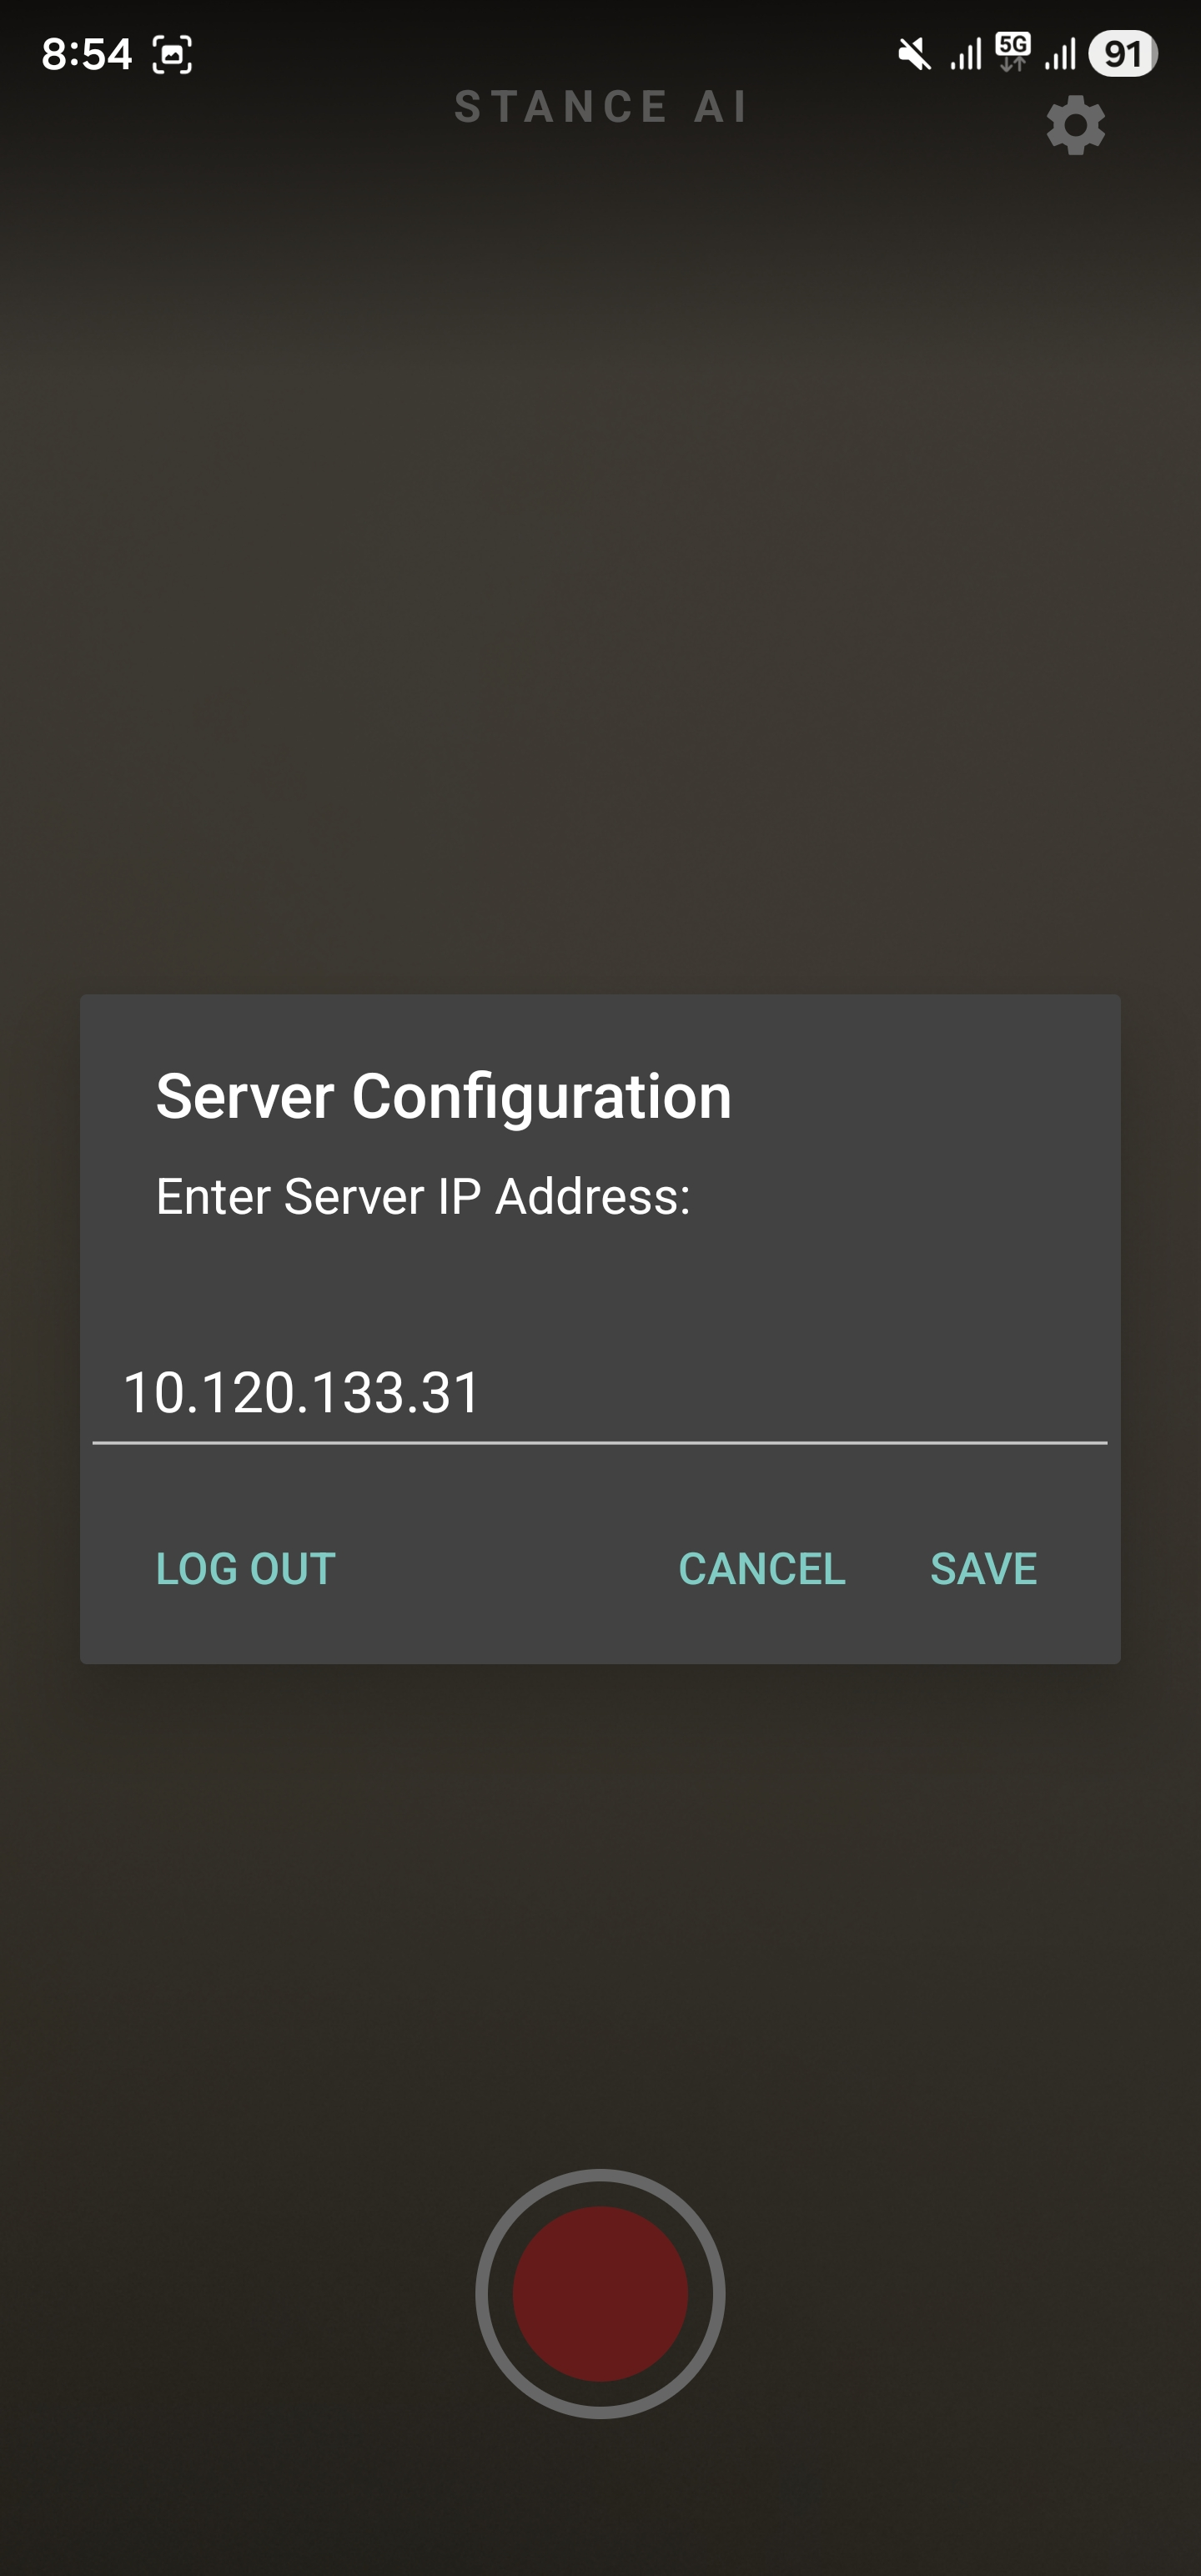
\includegraphics[width=0.27\linewidth]{Figures/Chapter-8figs/logout_page}
	\caption{Logout Page}
	\label{fig:logout}
\end{figure}

\subsection{Detection Result – CUT SHOT}
	
	The first image demonstrates the AI Cricket Coach system detecting a Cut Shot using the YOLOv8-based object detection model. In this frame, the system identifies the player’s body posture, bat alignment, arm extension, and follow-through direction through bounding boxes and pose estimation overlays. The blue bounding box highlights the detected person with a confidence score, while skeletal lines indicate key joint alignments used for classification. Based on bat angle, lateral arm movement, and upper-body rotation, the model classifies the stance as a Cut Shot. The detected stance label is displayed prominently at the bottom of the screen as “CUT SHOT.” This output confirms the system’s ability to analyze shot direction and technical posture in real time. The detection is processed on the backend server and returned to the Android application, where the result is displayed along with interactive options such as “Take Another Photo” for repeated analysis.
	
	\begin{figure}[H]
		\centering
		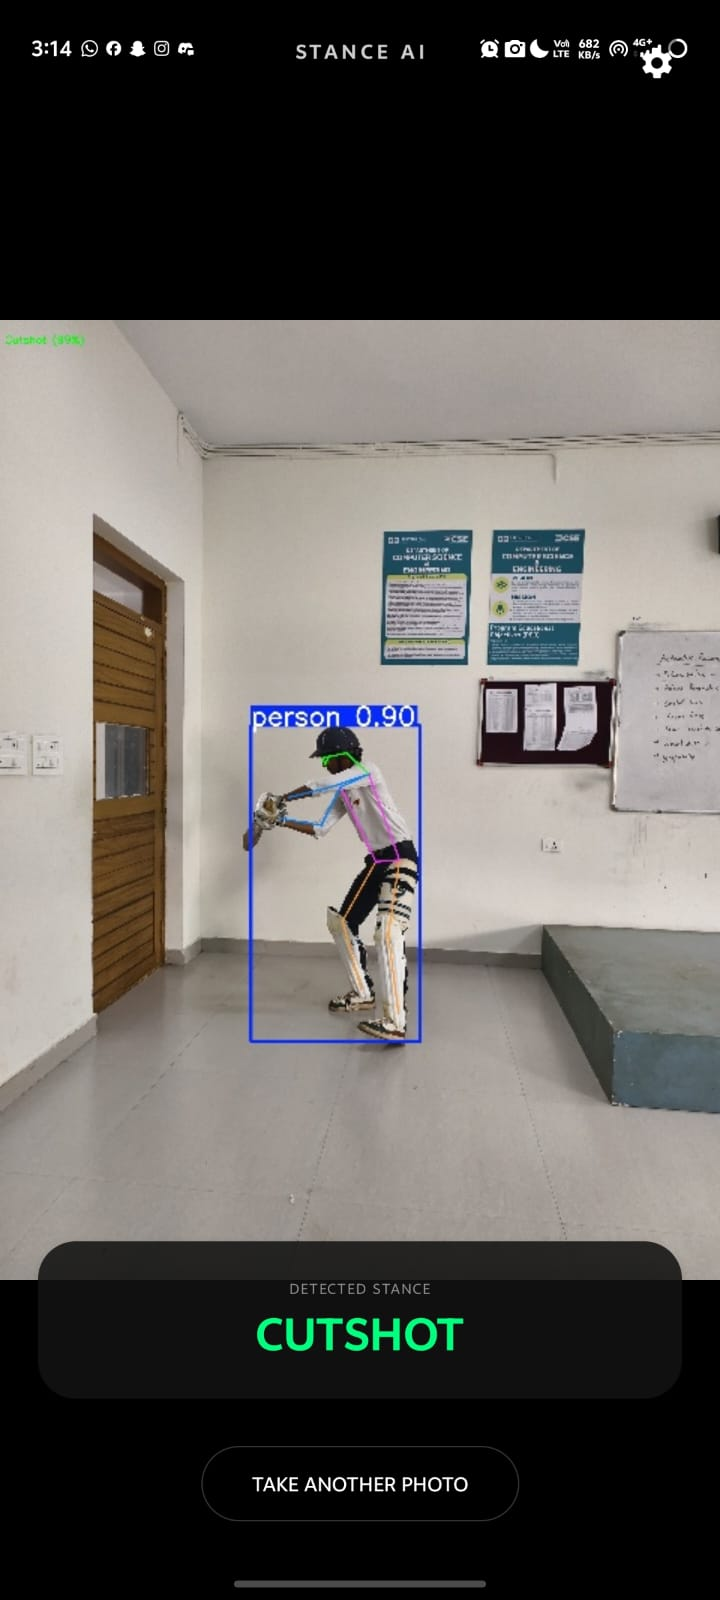
\includegraphics[width=0.32\linewidth]{Figures/Chapter-8figs/cutshot}
		\caption{Cut Shot}
		\label{fig:cutshot}
	\end{figure}
	
\subsection{Detection Result – PULL SHOT}
	
	The second image illustrates the AI Cricket Coach system detecting a Pull Shot. In this case, the player’s bat is raised horizontally across the body with a strong upper-body rotation, which is a defining characteristic of the pull shot technique. The YOLOv8 model detects the person and extracts spatial features such as bat orientation, shoulder alignment, and swing trajectory. These features are analyzed to determine the shot category. The bounding boxes display detection confidence levels, while pose lines help evaluate the correctness of execution. Once classified, the system displays “PULL SHOT” as the detected stance. The classification is further used by the integrated XGBoost regression model to compute a performance score based on shot stability and posture efficiency. This demonstrates the system’s capability to distinguish aggressive horizontal bat shots using advanced computer vision techniques.
	
	\begin{figure}[H]
		\centering
		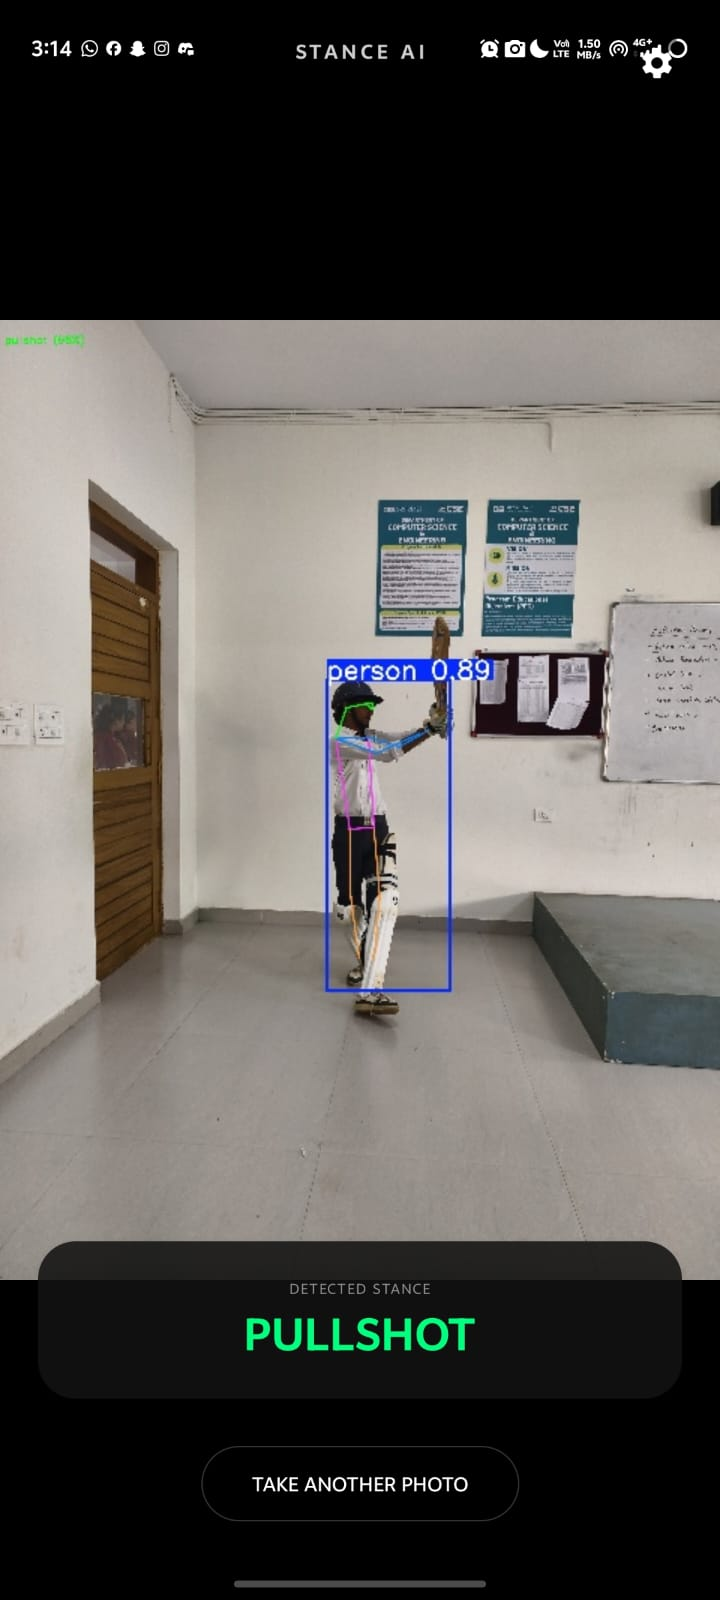
\includegraphics[width=0.32\linewidth]{Figures/Chapter-8figs/pullshot}
		\caption{Pull Shot}
		\label{fig:pullshot}
	\end{figure}
	
\subsection{Detection Result – SWEEP}
	
	The third image shows the AI Cricket Coach system identifying a Sweep Shot. In this scenario, the player bends forward with a low body stance and extended bat swing directed towards the leg side. The YOLOv8 model detects the person and analyzes lower-body positioning, knee bend, bat trajectory, and balance distribution. The skeletal overlay lines represent key joint tracking used for posture evaluation. The model classifies the stance as “SWEEP” based on these spatial features and movement orientation. The detected label is displayed at the bottom of the screen as confirmation of classification. This output demonstrates the system’s capability to recognize low sweeping strokes and differentiate them from vertical or horizontal bat shots. The classification result is processed in real time and presented to the user through the Android interface, enabling immediate feedback during practice sessions.
	
	\begin{figure}[H]
		\centering
		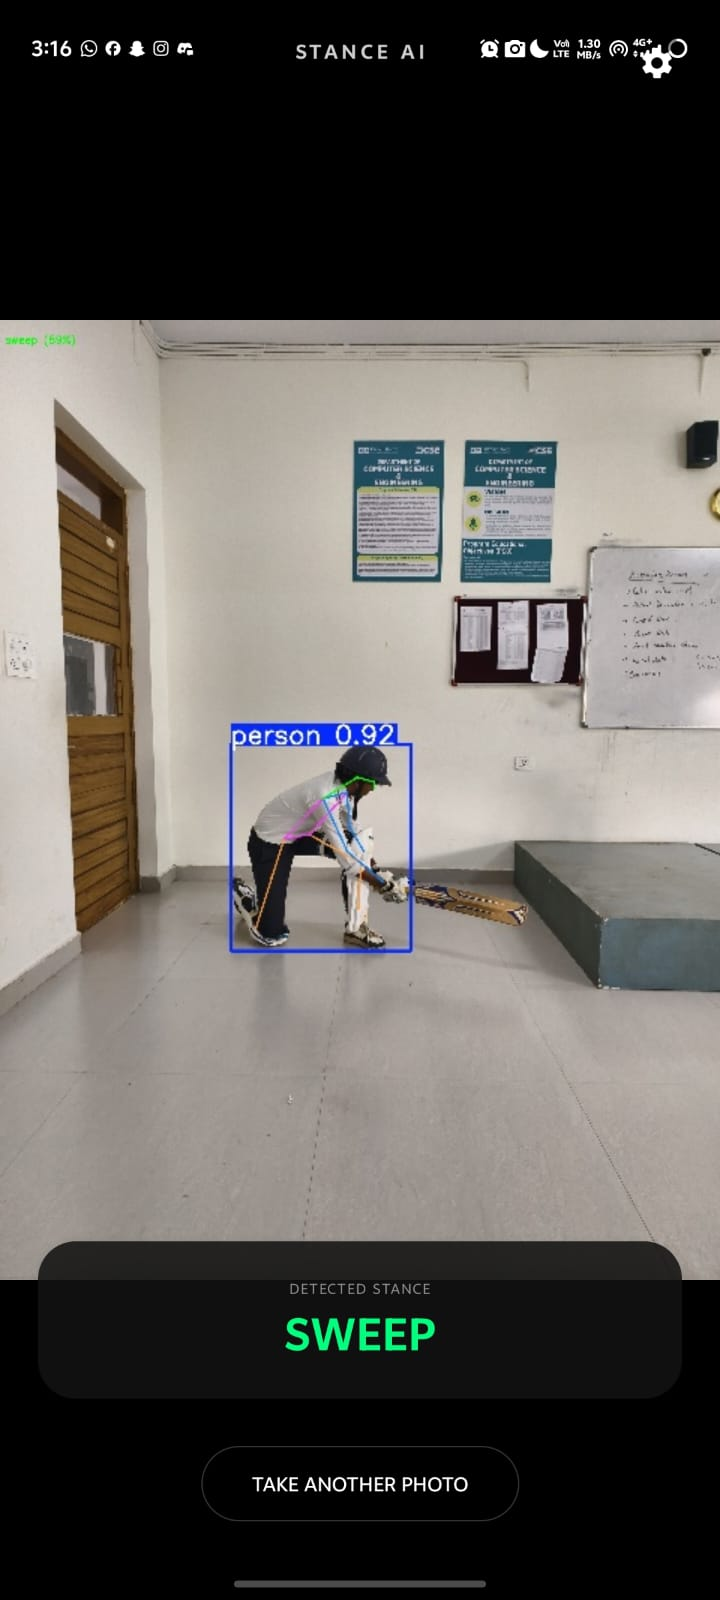
\includegraphics[width=0.32\linewidth]{Figures/Chapter-8figs/sweep}
		\caption{Sweep}
		\label{fig:sweep}
	\end{figure}
	
\subsection{Detection Result – STRAIGHT DRIVE}
	
	This image represents the AI Cricket Coach system detecting a Straight Drive using the YOLOv8-based object detection model integrated into the backend server. In this stance, the player maintains a balanced posture with a vertically aligned bat swing directed straight down the ground. The model identifies the player using bounding box detection and analyzes key spatial features such as bat angle, front-foot positioning, shoulder alignment, and follow-through direction. The skeletal overlay lines indicate joint tracking used to evaluate posture symmetry and technical correctness. Based on the near-vertical bat trajectory and forward body alignment, the system classifies the shot as a Straight Drive. The detected stance is displayed at the bottom of the screen as “STRAIGHT DRIVE.” After classification, extracted numerical features are passed to the XGBoost regression model to generate a performance score reflecting shot balance, bat control, and execution quality. This demonstrates the system’s ability to accurately recognize technically correct front-foot attacking strokes in real time.
	
	\begin{figure}[H]
		\centering
		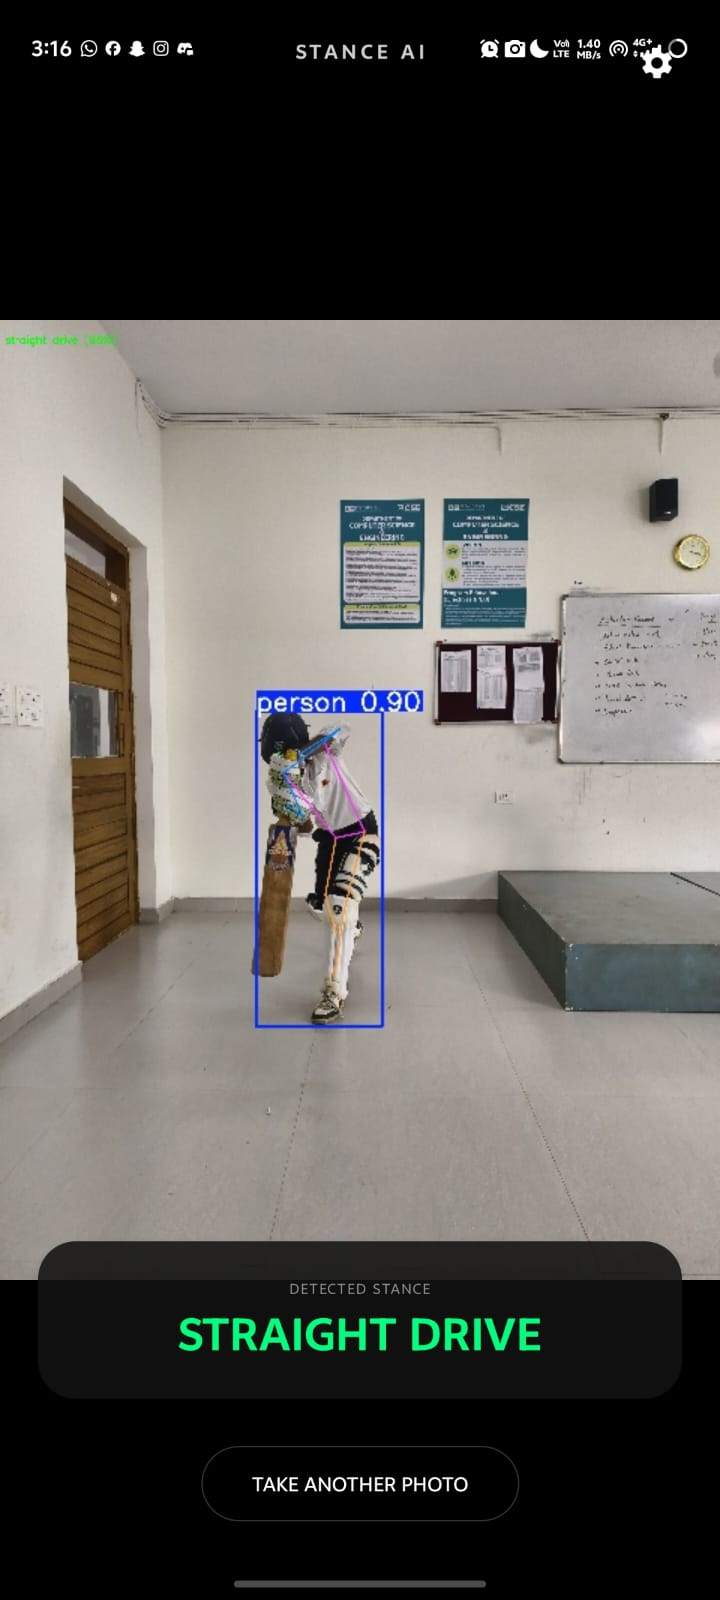
\includegraphics[width=0.32\linewidth]{Figures/Chapter-8figs/straight_drive}
		\caption{Straight Drive}
		\label{fig:straightdrive}
	\end{figure}
	
\subsection{Detection Result – UNKNOWN}
	
	This image illustrates a scenario where the AI Cricket Coach system classifies the stance as Unknown. The Unknown category is triggered when the detection confidence score falls below a predefined threshold or when the shot posture does not sufficiently match any of the trained categories such as Straight Drive, Pull Shot, Cut Shot, or Sweep Shot. The YOLOv8 model may detect the player and generate bounding boxes, but inconsistencies in bat angle, incomplete follow-through, improper framing, or ambiguous body positioning can reduce classification confidence. To minimize misclassification and maintain system reliability, a confidence threshold mechanism is implemented in the backend. If the prediction probability is below this threshold, the system labels the output as “UNKNOWN” instead of forcing an incorrect classification. This feature enhances the robustness of the AI Cricket Coach by ensuring that only reliable predictions are presented to the user. The Unknown classification encourages the user to retake the image for more accurate analysis and maintains the overall integrity of the model’s performance evaluation system.
	
	\begin{figure}[H]
		\centering
		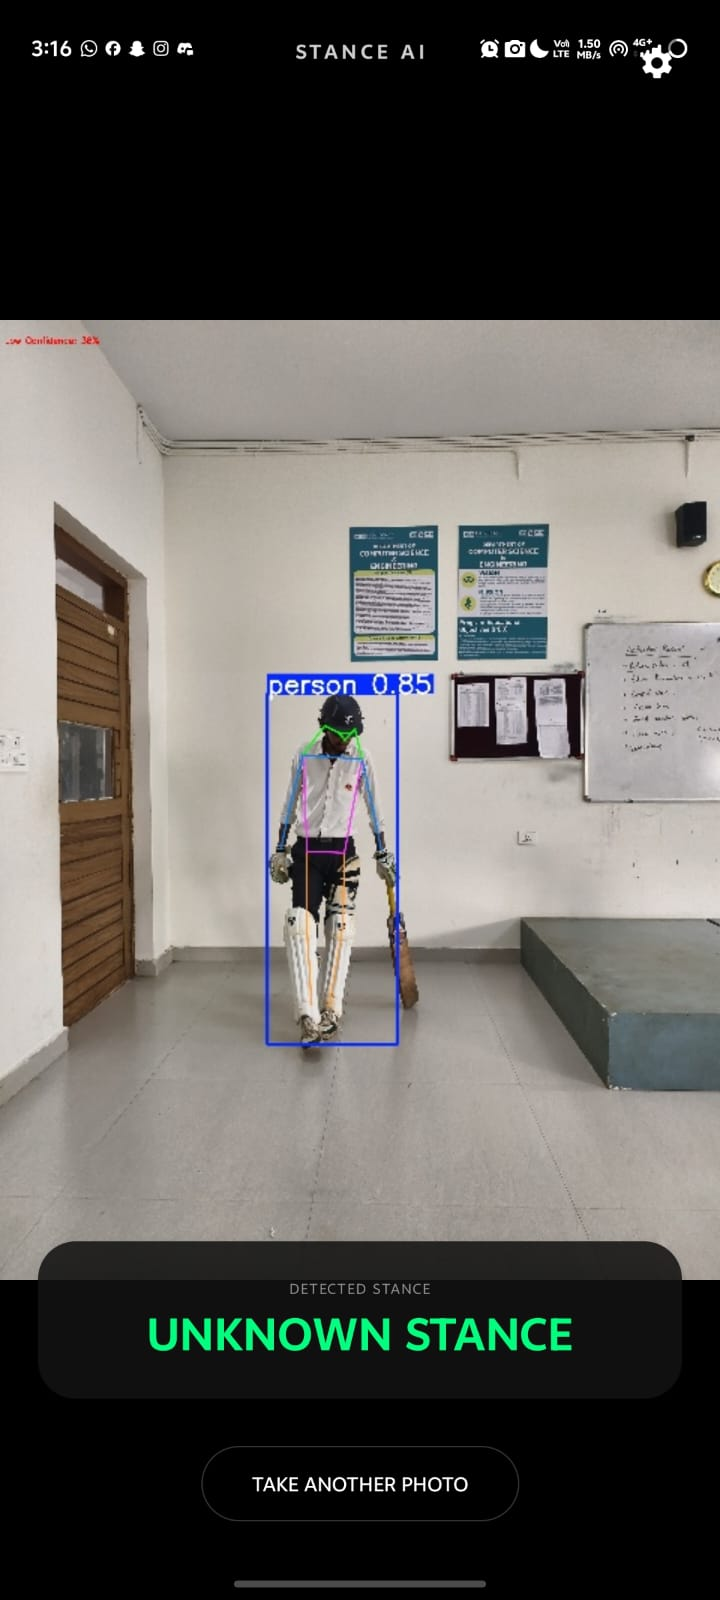
\includegraphics[width=0.32\linewidth]{Figures/Chapter-8figs/unknown_stance}
		\caption{Unknown Stance}
		\label{fig:unknown}
	\end{figure}
	
\subsection{Detection Result – NO PERSON DETECTED}
	
	This image represents a scenario in which the AI Cricket Coach system displays the result as “No Person Detected.” In this case, the YOLOv8 object detection model fails to identify any human subject within the captured frame. The system initially processes the input image by performing inference through the trained YOLOv8 model, which is configured to detect the “person” class along with relevant pose and spatial features. However, if the model does not detect a bounding box with sufficient confidence corresponding to a human subject, the system determines that no valid cricket stance can be analyzed.
	This situation may occur due to improper framing, absence of a player in the image, poor lighting conditions, motion blur, occlusion, or the subject being partially outside the camera frame. Since the AI Cricket Coach system relies on human body posture, bat alignment, and joint orientation for shot classification and performance evaluation, the absence of a detected person prevents further processing. In such cases, the backend server bypasses the classification and regression modules and returns a structured response indicating “No Person Detected.” The Android application then displays this result to the user and prompts them to capture another image. This validation mechanism ensures that the system does not attempt incorrect shot classification or generate invalid performance scores when essential detection criteria are not met. The inclusion of the “No Person Detected” condition enhances system robustness, reliability, and user guidance during real-time cricket practice sessions.
	
	\begin{figure}[H]
		\centering
		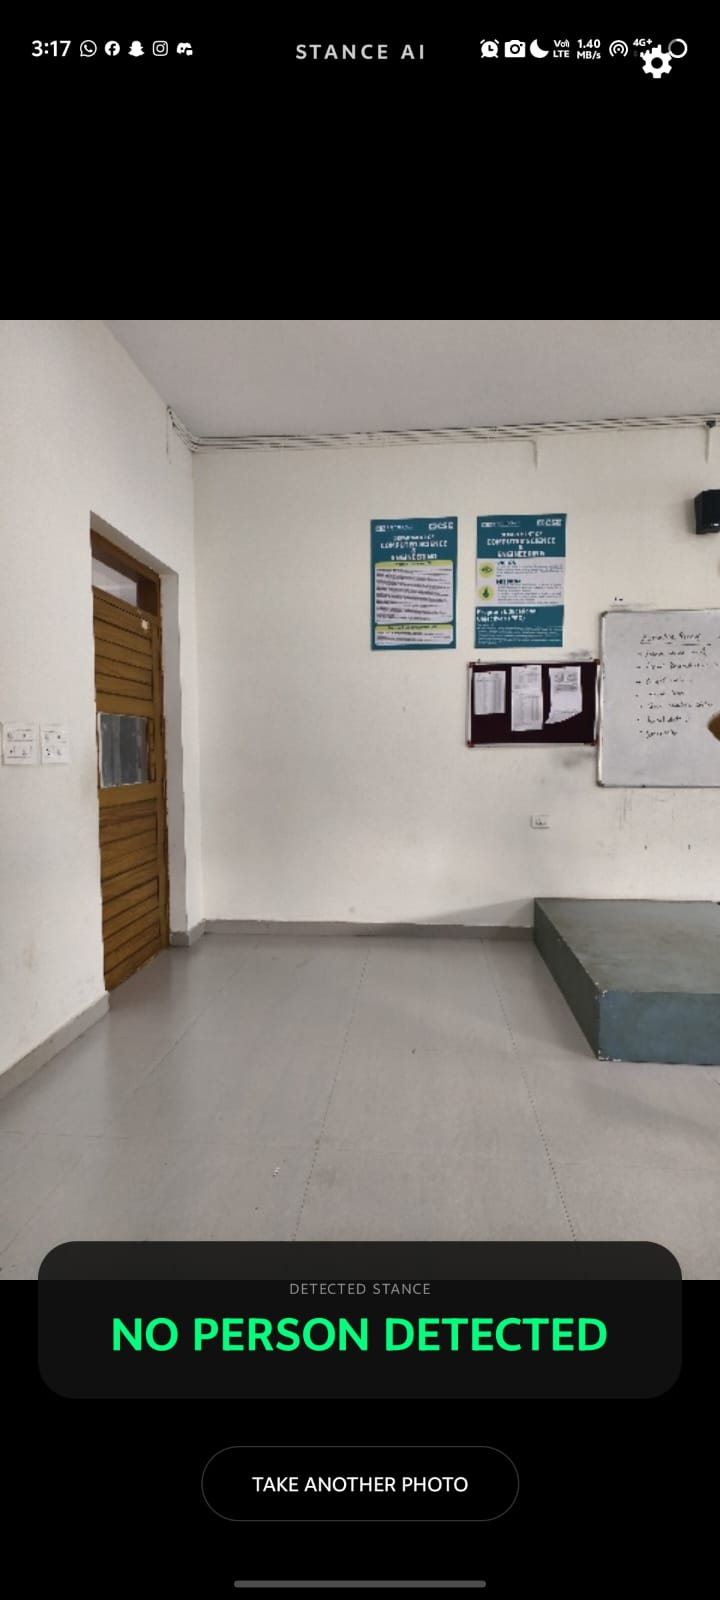
\includegraphics[width=0.32\linewidth]{Figures/Chapter-8figs/no_detection}
		\caption{No Person Detected}
		\label{fig:nodetection}
	\end{figure}
	
\section{Performance Evaluation Results}
    \begin{table}[h]
    	\centering
    	\caption{Performance Metrics for Cricket Shot Classification Model}
    	\label{tab:results}
    	
    	\resizebox{0.7\textwidth}{!}{
    		\begin{tabular}{|l|c|c|c|}
    			\hline
    			\rowcolor{gray!30}
    			\textbf{Shot Class} & \textbf{Precision} & \textbf{Recall} & \textbf{Accuracy} \\
    			\hline
    			Straight Drive & 0.94 & 0.92 & 0.93 \\
    			\hline
    			Pull Shot      & 0.91 & 0.90 & 0.91 \\
    			\hline
    			Cut Shot       & 0.93 & 0.95 & 0.94 \\
    			\hline
    			Sweep          & 0.90 & 0.88 & 0.89 \\
    			\hline
    			Unknown        & 0.88 & 0.87 & 0.87 \\
    			\hline
    			No Detection   & 0.82 & 0.90 & 0.94 \\
    			\hline
    		\end{tabular}
    	}
    	
    \end{table}
    
    The table 8.1 shows the performance of the cricket shot classification system using key evaluation metrics such as precision, recall, and accuracy. Each shot type Straight Drive, Pull Shot, Cut Shot, and Sweep has been evaluated separately to understand how well the model distinguishes between different batting techniques. The results show that the model performs consistently across all classes, with high accuracy values indicating reliable predictions. The “Unknown” category is used when the model is not confident or when the input does not match any trained class, which helps reduce incorrect classifications. In addition, the “No Detection” case represents situations where no player is present in the image, and the system correctly identifies this condition. This scenario is treated separately to evaluate the detection capability of the system. Overall, the results suggest that the model is capable of delivering stable and accurate predictions, making it suitable for real-time cricket training and analysis applications.